\documentclass[10pt,a4paper,onecolumn]{article}
\usepackage{marginnote}
\usepackage{graphicx}
\usepackage[rgb,svgnames]{xcolor}
\usepackage{authblk,etoolbox}
\usepackage{titlesec}
\usepackage{calc}
\usepackage{tikz}
\usepackage[pdfa]{hyperref}
\usepackage{hyperxmp}
\hypersetup{%
    unicode=true,
    pdfapart=3,
    pdfaconformance=B,
    pdftitle={maze-dataset},
    pdfauthor={Michael Igorevich Ivanitskiy, Aaron Sandoval, Alex F.
Spies, Rusheb Shah, Brandon Knutson, , Cecilia Diniz Behn, Samy Wu
Fung},
    pdfpublication={Journal of Open Source Software},
    pdfpublisher={Open Journals},
    pdfissn={2475-9066},
    pdfpubtype={journal},
    pdfvolumenum={},
    pdfissuenum={},
    pdfdoi={N/A},
    pdfcopyright={Copyright (c) 1970, Michael Igorevich Ivanitskiy,
Aaron Sandoval, Alex F. Spies, Rusheb Shah, Brandon Knutson, , Cecilia
Diniz Behn, Samy Wu Fung},
    pdflicenseurl={http://creativecommons.org/licenses/by/4.0/},
    colorlinks=true,
    linkcolor=[rgb]{0.0, 0.5, 1.0},
    citecolor=Blue,
    urlcolor=[rgb]{0.0, 0.5, 1.0},
    breaklinks=true
}
% https://tex.stackexchange.com/a/535849
% Create an OutputIntent in order to correctly specify colours
\immediate\pdfobj stream attr{/N 3} file{sRGB.icc}
\pdfcatalog{%
  /OutputIntents [
    <<
      /Type /OutputIntent
      /S /GTS_PDFA1
      /DestOutputProfile \the\pdflastobj\space 0 R
      /OutputConditionIdentifier (sRGB)
      /Info (sRGB)
    >>
  ]
}
\pdfvariable omitcidset=1
\usepackage{caption}
\usepackage{orcidlink}
\usepackage{tcolorbox}
\usepackage{amssymb,amsmath}
\usepackage{ifxetex,ifluatex}
\usepackage{seqsplit}
\usepackage{xstring}

\usepackage{float}
\let\origfigure\figure
\let\endorigfigure\endfigure
\renewenvironment{figure}[1][2] {
    \expandafter\origfigure\expandafter[H]
} {
    \endorigfigure
}

\usepackage{fixltx2e} % provides \textsubscript

% definitions for citeproc citations
\NewDocumentCommand\citeproctext{}{}
\NewDocumentCommand\citeproc{mm}{%
  \begingroup\def\citeproctext{#2}\cite{#1}\endgroup}
\makeatletter
 % allow citations to break across lines
 \let\@cite@ofmt\@firstofone
 % avoid brackets around text for \cite:
 \def\@biblabel#1{}
 \def\@cite#1#2{{#1\if@tempswa , #2\fi}}
\makeatother
\newlength{\cslhangindent}
\setlength{\cslhangindent}{1.5em}
\newlength{\csllabelwidth}
\setlength{\csllabelwidth}{3em}
\newenvironment{CSLReferences}[2] % #1 hanging-indent, #2 entry-spacing
 {\begin{list}{}{%
  \setlength{\itemindent}{0pt}
  \setlength{\leftmargin}{0pt}
  \setlength{\parsep}{0pt}
  % turn on hanging indent if param 1 is 1
  \ifodd #1
   \setlength{\leftmargin}{\cslhangindent}
   \setlength{\itemindent}{-1\cslhangindent}
  \fi
  % set entry spacing
  \setlength{\itemsep}{#2\baselineskip}}}
 {\end{list}}
\usepackage{calc}
\newcommand{\CSLBlock}[1]{\hfill\break\parbox[t]{\linewidth}{\strut\ignorespaces#1\strut}}
\newcommand{\CSLLeftMargin}[1]{\parbox[t]{\csllabelwidth}{\strut#1\strut}}
\newcommand{\CSLRightInline}[1]{\parbox[t]{\linewidth - \csllabelwidth}{\strut#1\strut}}
\newcommand{\CSLIndent}[1]{\hspace{\cslhangindent}#1}

% --- Page layout -------------------------------------------------------------
\usepackage[top=3.5cm, bottom=3cm, right=1.5cm, left=1.0cm,
            headheight=2.2cm, reversemp, includemp, marginparwidth=4.5cm]{geometry}

% --- Default font ------------------------------------------------------------
\renewcommand\familydefault{\sfdefault}

% --- Style -------------------------------------------------------------------
\renewcommand{\captionfont}{\small\sffamily}
\renewcommand{\captionlabelfont}{\bfseries}

% --- Section/SubSection/SubSubSection ----------------------------------------
\titleformat{\section}
  {\normalfont\sffamily\Large\bfseries}
  {}{0pt}{}
\titleformat{\subsection}
  {\normalfont\sffamily\large\bfseries}
  {}{0pt}{}
\titleformat{\subsubsection}
  {\normalfont\sffamily\bfseries}
  {}{0pt}{}
\titleformat*{\paragraph}
  {\sffamily\normalsize}


% --- Header / Footer ---------------------------------------------------------
\usepackage{fancyhdr}
\pagestyle{fancy}
\fancyhf{}
%\renewcommand{\headrulewidth}{0.50pt}
\renewcommand{\headrulewidth}{0pt}
\fancyhead[L]{\hspace{-0.75cm}
\includegraphics[width=5.5cm]{joss/logo.png}}
\fancyhead[C]{}
\fancyhead[R]{}
\renewcommand{\footrulewidth}{0.25pt}

\fancyfoot[L]{\parbox[t]{0.98\headwidth}{\footnotesize{\sffamily Ivanitskiy
et al. (1970). maze-dataset. \emph{Journal of Open Source Software},
\emph{¿VOL?}(¿ISSUE?), ¿PAGE? \url{https://doi.org/N/A}}.}}


\fancyfoot[R]{\sffamily \thepage}
\makeatletter
\let\ps@plain\ps@fancy
\fancyheadoffset[L]{4.5cm}
\fancyfootoffset[L]{4.5cm}

% --- Macros ---------

\definecolor{linky}{rgb}{0.0, 0.5, 1.0}

\newtcolorbox{repobox}
   {colback=red, colframe=red!75!black,
     boxrule=0.5pt, arc=2pt, left=6pt, right=6pt, top=3pt, bottom=3pt}

\newcommand{\ExternalLink}{%
   \tikz[x=1.2ex, y=1.2ex, baseline=-0.05ex]{%
       \begin{scope}[x=1ex, y=1ex]
           \clip (-0.1,-0.1)
               --++ (-0, 1.2)
               --++ (0.6, 0)
               --++ (0, -0.6)
               --++ (0.6, 0)
               --++ (0, -1);
           \path[draw,
               line width = 0.5,
               rounded corners=0.5]
               (0,0) rectangle (1,1);
       \end{scope}
       \path[draw, line width = 0.5] (0.5, 0.5)
           -- (1, 1);
       \path[draw, line width = 0.5] (0.6, 1)
           -- (1, 1) -- (1, 0.6);
       }
   }

\definecolor{c53baa1}{RGB}{83,186,161}
\definecolor{c202826}{RGB}{32,40,38}
\def \rorglobalscale {0.1}
\newcommand{\rorlogo}{%
\begin{tikzpicture}[y=1cm, x=1cm, yscale=\rorglobalscale,xscale=\rorglobalscale, every node/.append style={scale=\rorglobalscale}, inner sep=0pt, outer sep=0pt]
  \begin{scope}[even odd rule,line join=round,miter limit=2.0,shift={(-0.025, 0.0216)}]
    \path[fill=c53baa1,nonzero rule,line join=round,miter limit=2.0] (1.8164, 3.012) -- (1.4954, 2.5204) -- (1.1742, 3.012) -- (1.8164, 3.012) -- cycle;
    \path[fill=c53baa1,nonzero rule,line join=round,miter limit=2.0] (3.1594, 3.012) -- (2.8385, 2.5204) -- (2.5172, 3.012) -- (3.1594, 3.012) -- cycle;
    \path[fill=c53baa1,nonzero rule,line join=round,miter limit=2.0] (1.1742, 0.0669) -- (1.4954, 0.5588) -- (1.8164, 0.0669) -- (1.1742, 0.0669) -- cycle;
    \path[fill=c53baa1,nonzero rule,line join=round,miter limit=2.0] (2.5172, 0.0669) -- (2.8385, 0.5588) -- (3.1594, 0.0669) -- (2.5172, 0.0669) -- cycle;
    \path[fill=c202826,nonzero rule,line join=round,miter limit=2.0] (3.8505, 1.4364).. controls (3.9643, 1.4576) and (4.0508, 1.5081) .. (4.1098, 1.5878).. controls (4.169, 1.6674) and (4.1984, 1.7642) .. (4.1984, 1.8777).. controls (4.1984, 1.9719) and (4.182, 2.0503) .. (4.1495, 2.1132).. controls (4.1169, 2.1762) and (4.0727, 2.2262) .. (4.0174, 2.2635).. controls (3.9621, 2.3006) and (3.8976, 2.3273) .. (3.824, 2.3432).. controls (3.7505, 2.359) and (3.6727, 2.367) .. (3.5909, 2.367) -- (2.9676, 2.367) -- (2.9676, 1.8688).. controls (2.9625, 1.8833) and (2.9572, 1.8976) .. (2.9514, 1.9119).. controls (2.9083, 2.0164) and (2.848, 2.1056) .. (2.7705, 2.1791).. controls (2.6929, 2.2527) and (2.6014, 2.3093) .. (2.495, 2.3487).. controls (2.3889, 2.3881) and (2.2728, 2.408) .. (2.1468, 2.408).. controls (2.0209, 2.408) and (1.905, 2.3881) .. (1.7986, 2.3487).. controls (1.6925, 2.3093) and (1.6007, 2.2527) .. (1.5232, 2.1791).. controls (1.4539, 2.1132) and (1.3983, 2.0346) .. (1.3565, 1.9436).. controls (1.3504, 2.009) and (1.3351, 2.0656) .. (1.3105, 2.1132).. controls (1.2779, 2.1762) and (1.2338, 2.2262) .. (1.1785, 2.2635).. controls (1.1232, 2.3006) and (1.0586, 2.3273) .. (0.985, 2.3432).. controls (0.9115, 2.359) and (0.8337, 2.367) .. (0.7519, 2.367) -- (0.1289, 2.367) -- (0.1289, 0.7562) -- (0.4837, 0.7562) -- (0.4837, 1.4002) -- (0.6588, 1.4002) -- (0.9956, 0.7562) -- (1.4211, 0.7562) -- (1.0118, 1.4364).. controls (1.1255, 1.4576) and (1.2121, 1.5081) .. (1.2711, 1.5878).. controls (1.2737, 1.5915) and (1.2761, 1.5954) .. (1.2787, 1.5991).. controls (1.2782, 1.5867) and (1.2779, 1.5743) .. (1.2779, 1.5616).. controls (1.2779, 1.4327) and (1.2996, 1.3158) .. (1.3428, 1.2113).. controls (1.3859, 1.1068) and (1.4462, 1.0176) .. (1.5237, 0.944).. controls (1.601, 0.8705) and (1.6928, 0.8139) .. (1.7992, 0.7744).. controls (1.9053, 0.735) and (2.0214, 0.7152) .. (2.1474, 0.7152).. controls (2.2733, 0.7152) and (2.3892, 0.735) .. (2.4956, 0.7744).. controls (2.6016, 0.8139) and (2.6935, 0.8705) .. (2.771, 0.944).. controls (2.8482, 1.0176) and (2.9086, 1.1068) .. (2.952, 1.2113).. controls (2.9578, 1.2253) and (2.9631, 1.2398) .. (2.9681, 1.2544) -- (2.9681, 0.7562) -- (3.3229, 0.7562) -- (3.3229, 1.4002) -- (3.4981, 1.4002) -- (3.8349, 0.7562) -- (4.2603, 0.7562) -- (3.8505, 1.4364) -- cycle(0.9628, 1.7777).. controls (0.9438, 1.7534) and (0.92, 1.7357) .. (0.8911, 1.7243).. controls (0.8623, 1.7129) and (0.83, 1.706) .. (0.7945, 1.7039).. controls (0.7588, 1.7015) and (0.7252, 1.7005) .. (0.6932, 1.7005) -- (0.4839, 1.7005) -- (0.4839, 2.0667) -- (0.716, 2.0667).. controls (0.7477, 2.0667) and (0.7805, 2.0643) .. (0.8139, 2.0598).. controls (0.8472, 2.0553) and (0.8768, 2.0466) .. (0.9025, 2.0336).. controls (0.9282, 2.0206) and (0.9496, 2.0021) .. (0.9663, 1.9778).. controls (0.9829, 1.9534) and (0.9914, 1.9209) .. (0.9914, 1.8799).. controls (0.9914, 1.8362) and (0.9819, 1.8021) .. (0.9628, 1.7777) -- cycle(2.6125, 1.3533).. controls (2.5889, 1.2904) and (2.5553, 1.2359) .. (2.5112, 1.1896).. controls (2.4672, 1.1433) and (2.4146, 1.1073) .. (2.3529, 1.0814).. controls (2.2916, 1.0554) and (2.2228, 1.0427) .. (2.1471, 1.0427).. controls (2.0712, 1.0427) and (2.0026, 1.0557) .. (1.9412, 1.0814).. controls (1.8799, 1.107) and (1.8272, 1.1433) .. (1.783, 1.1896).. controls (1.7391, 1.2359) and (1.7052, 1.2904) .. (1.6817, 1.3533).. controls (1.6581, 1.4163) and (1.6465, 1.4856) .. (1.6465, 1.5616).. controls (1.6465, 1.6359) and (1.6581, 1.705) .. (1.6817, 1.7687).. controls (1.7052, 1.8325) and (1.7388, 1.8873) .. (1.783, 1.9336).. controls (1.8269, 1.9799) and (1.8796, 2.0159) .. (1.9412, 2.0418).. controls (2.0026, 2.0675) and (2.0712, 2.0804) .. (2.1471, 2.0804).. controls (2.223, 2.0804) and (2.2916, 2.0675) .. (2.3529, 2.0418).. controls (2.4143, 2.0161) and (2.467, 1.9799) .. (2.5112, 1.9336).. controls (2.5551, 1.8873) and (2.5889, 1.8322) .. (2.6125, 1.7687).. controls (2.636, 1.705) and (2.6477, 1.6359) .. (2.6477, 1.5616).. controls (2.6477, 1.4856) and (2.636, 1.4163) .. (2.6125, 1.3533) -- cycle(3.8015, 1.7777).. controls (3.7825, 1.7534) and (3.7587, 1.7357) .. (3.7298, 1.7243).. controls (3.701, 1.7129) and (3.6687, 1.706) .. (3.6333, 1.7039).. controls (3.5975, 1.7015) and (3.5639, 1.7005) .. (3.5319, 1.7005) -- (3.3226, 1.7005) -- (3.3226, 2.0667) -- (3.5547, 2.0667).. controls (3.5864, 2.0667) and (3.6192, 2.0643) .. (3.6526, 2.0598).. controls (3.6859, 2.0553) and (3.7155, 2.0466) .. (3.7412, 2.0336).. controls (3.7669, 2.0206) and (3.7883, 2.0021) .. (3.805, 1.9778).. controls (3.8216, 1.9534) and (3.8301, 1.9209) .. (3.8301, 1.8799).. controls (3.8301, 1.8362) and (3.8206, 1.8021) .. (3.8015, 1.7777) -- cycle;
  \end{scope}
\end{tikzpicture}
}

% --- Title / Authors ---------------------------------------------------------
% patch \maketitle so that it doesn't center
\patchcmd{\@maketitle}{center}{flushleft}{}{}
\patchcmd{\@maketitle}{center}{flushleft}{}{}
% patch \maketitle so that the font size for the title is normal
\patchcmd{\@maketitle}{\LARGE}{\LARGE\sffamily}{}{}
% patch the patch by authblk so that the author block is flush left
\def\maketitle{{%
  \renewenvironment{tabular}[2][]
    {\begin{flushleft}}
    {\end{flushleft}}
  \AB@maketitle}}
\renewcommand\AB@affilsepx{ \protect\Affilfont}
%\renewcommand\AB@affilnote[1]{{\bfseries #1}\hspace{2pt}}
\renewcommand\AB@affilnote[1]{{\bfseries #1}\hspace{3pt}}
\renewcommand{\affil}[2][]%
   {\newaffiltrue\let\AB@blk@and\AB@pand
      \if\relax#1\relax\def\AB@note{\AB@thenote}\else\def\AB@note{#1}%
        \setcounter{Maxaffil}{0}\fi
        \begingroup
        \let\href=\href@Orig
        \let\protect\@unexpandable@protect
        \def\thanks{\protect\thanks}\def\footnote{\protect\footnote}%
        \@temptokena=\expandafter{\AB@authors}%
        {\def\\{\protect\\\protect\Affilfont}\xdef\AB@temp{#2}}%
         \xdef\AB@authors{\the\@temptokena\AB@las\AB@au@str
         \protect\\[\affilsep]\protect\Affilfont\AB@temp}%
         \gdef\AB@las{}\gdef\AB@au@str{}%
        {\def\\{, \ignorespaces}\xdef\AB@temp{#2}}%
        \@temptokena=\expandafter{\AB@affillist}%
        \xdef\AB@affillist{\the\@temptokena \AB@affilsep
          \AB@affilnote{\AB@note}\protect\Affilfont\AB@temp}%
      \endgroup
       \let\AB@affilsep\AB@affilsepx
}
\makeatother
\renewcommand\Authfont{\sffamily\bfseries}
\renewcommand\Affilfont{\sffamily\small\mdseries}
\setlength{\affilsep}{1em}


\ifnum 0\ifxetex 1\fi\ifluatex 1\fi=0 % if pdftex
  \usepackage[T1]{fontenc}
  \usepackage[utf8]{inputenc}

\else % if luatex or xelatex
  \ifxetex
    \usepackage{mathspec}
    \usepackage{fontspec}

  \else
    \usepackage{fontspec}
  \fi
  \defaultfontfeatures{Scale=MatchLowercase}
  \defaultfontfeatures[\sffamily]{Ligatures=TeX}
  \defaultfontfeatures[\rmfamily]{Ligatures=TeX,Scale=1}

\fi
% use upquote if available, for straight quotes in verbatim environments
\IfFileExists{upquote.sty}{\usepackage{upquote}}{}
% use microtype if available
\IfFileExists{microtype.sty}{%
\usepackage{microtype}
\UseMicrotypeSet[protrusion]{basicmath} % disable protrusion for tt fonts
}{}

%% Font settings
\usepackage{fontsetup} % Lazy way to get proper Greek lowercase glyphs

% Use Hack https://sourcefoundry.org/hack/
\setmonofont{Hack}

\PassOptionsToPackage{usenames,dvipsnames}{color} % color is loaded by hyperref
\urlstyle{same}  % don't use monospace font for urls
\ifLuaTeX
\usepackage[bidi=basic]{babel}
\else
\usepackage[bidi=default]{babel}
\fi
\babelprovide[main,import]{american}
% get rid of language-specific shorthands (see #6817):
\let\LanguageShortHands\languageshorthands
\def\languageshorthands#1{}
\usepackage{color}
\usepackage{fancyvrb}
\newcommand{\VerbBar}{|}
\newcommand{\VERB}{\Verb[commandchars=\\\{\}]}
\DefineVerbatimEnvironment{Highlighting}{Verbatim}{commandchars=\\\{\}}
% Add ',fontsize=\small' for more characters per line
\newenvironment{Shaded}{}{}
\newcommand{\AlertTok}[1]{\textcolor[rgb]{1.00,0.00,0.00}{\textbf{#1}}}
\newcommand{\AnnotationTok}[1]{\textcolor[rgb]{0.38,0.63,0.69}{\textbf{\textit{#1}}}}
\newcommand{\AttributeTok}[1]{\textcolor[rgb]{0.49,0.56,0.16}{#1}}
\newcommand{\BaseNTok}[1]{\textcolor[rgb]{0.25,0.63,0.44}{#1}}
\newcommand{\BuiltInTok}[1]{\textcolor[rgb]{0.00,0.50,0.00}{#1}}
\newcommand{\CharTok}[1]{\textcolor[rgb]{0.25,0.44,0.63}{#1}}
\newcommand{\CommentTok}[1]{\textcolor[rgb]{0.38,0.63,0.69}{\textit{#1}}}
\newcommand{\CommentVarTok}[1]{\textcolor[rgb]{0.38,0.63,0.69}{\textbf{\textit{#1}}}}
\newcommand{\ConstantTok}[1]{\textcolor[rgb]{0.53,0.00,0.00}{#1}}
\newcommand{\ControlFlowTok}[1]{\textcolor[rgb]{0.00,0.44,0.13}{\textbf{#1}}}
\newcommand{\DataTypeTok}[1]{\textcolor[rgb]{0.56,0.13,0.00}{#1}}
\newcommand{\DecValTok}[1]{\textcolor[rgb]{0.25,0.63,0.44}{#1}}
\newcommand{\DocumentationTok}[1]{\textcolor[rgb]{0.73,0.13,0.13}{\textit{#1}}}
\newcommand{\ErrorTok}[1]{\textcolor[rgb]{1.00,0.00,0.00}{\textbf{#1}}}
\newcommand{\ExtensionTok}[1]{#1}
\newcommand{\FloatTok}[1]{\textcolor[rgb]{0.25,0.63,0.44}{#1}}
\newcommand{\FunctionTok}[1]{\textcolor[rgb]{0.02,0.16,0.49}{#1}}
\newcommand{\ImportTok}[1]{\textcolor[rgb]{0.00,0.50,0.00}{\textbf{#1}}}
\newcommand{\InformationTok}[1]{\textcolor[rgb]{0.38,0.63,0.69}{\textbf{\textit{#1}}}}
\newcommand{\KeywordTok}[1]{\textcolor[rgb]{0.00,0.44,0.13}{\textbf{#1}}}
\newcommand{\NormalTok}[1]{#1}
\newcommand{\OperatorTok}[1]{\textcolor[rgb]{0.40,0.40,0.40}{#1}}
\newcommand{\OtherTok}[1]{\textcolor[rgb]{0.00,0.44,0.13}{#1}}
\newcommand{\PreprocessorTok}[1]{\textcolor[rgb]{0.74,0.48,0.00}{#1}}
\newcommand{\RegionMarkerTok}[1]{#1}
\newcommand{\SpecialCharTok}[1]{\textcolor[rgb]{0.25,0.44,0.63}{#1}}
\newcommand{\SpecialStringTok}[1]{\textcolor[rgb]{0.73,0.40,0.53}{#1}}
\newcommand{\StringTok}[1]{\textcolor[rgb]{0.25,0.44,0.63}{#1}}
\newcommand{\VariableTok}[1]{\textcolor[rgb]{0.10,0.09,0.49}{#1}}
\newcommand{\VerbatimStringTok}[1]{\textcolor[rgb]{0.25,0.44,0.63}{#1}}
\newcommand{\WarningTok}[1]{\textcolor[rgb]{0.38,0.63,0.69}{\textbf{\textit{#1}}}}
\usepackage{longtable,booktabs,array}

\usepackage{graphicx,grffile}
\makeatletter
\def\maxwidth{\ifdim\Gin@nat@width>\linewidth\linewidth\else\Gin@nat@width\fi}
\def\maxheight{\ifdim\Gin@nat@height>\textheight\textheight\else\Gin@nat@height\fi}
\makeatother
% Scale images if necessary, so that they will not overflow the page
% margins by default, and it is still possible to overwrite the defaults
% using explicit options in \includegraphics[width, height, ...]{}
\setkeys{Gin}{width=\maxwidth,height=\maxheight,keepaspectratio}
\IfFileExists{parskip.sty}{%
\usepackage{parskip}
}{% else
\setlength{\parindent}{0pt}
\setlength{\parskip}{6pt plus 2pt minus 1pt}
}
\setlength{\emergencystretch}{3em}  % prevent overfull lines
\providecommand{\tightlist}{%
  \setlength{\itemsep}{0pt}\setlength{\parskip}{0pt}}
\setcounter{secnumdepth}{0}
% Redefines (sub)paragraphs to behave more like sections
\ifx\paragraph\undefined\else
\let\oldparagraph\paragraph
\renewcommand{\paragraph}[1]{\oldparagraph{#1}\mbox{}}
\fi
\ifx\subparagraph\undefined\else
\let\oldsubparagraph\subparagraph
\renewcommand{\subparagraph}[1]{\oldsubparagraph{#1}\mbox{}}
\fi
\usepackage{graphicx}
\usepackage{tikz}
\usepackage[luatex, pdfversion=1.7]{hyperref}
\usetikzlibrary{calc}
\tikzset{ % Define a TikZ style for an external hyperlink node.
  hyperlink node url/.style={
    alias=sourcenode,
    append after command={
      let \p1 = (sourcenode.north west),
          \p2 = (sourcenode.south east),
          \n1 = {\x2-\x1},
          \n2 = {\y1-\y2} in
      node[inner sep=0pt, outer sep=0pt, anchor=north west, at=(\p1)]
          {\href{#1}{\XeTeXLinkBox{\phantom{\rule{\n1}{\n2}}}}}
    }
  }
}
\providecommand{\XeTeXLinkBox}[1]{#1}
\ifLuaTeX
  \usepackage{selnolig}  % disable illegal ligatures
\fi

\title{maze-dataset}

\author[1%
%
\ensuremath\mathparagraph]{Michael Igorevich Ivanitskiy%
  \,\orcidlink{0000-0002-4213-4993}\,%
}
\author[%
%
]{Aaron Sandoval%
  \,\orcidlink{0009-0002-8380-6140}\,%
}
\author[2%
%
]{Alex F. Spies%
  \,\orcidlink{0000-0002-8708-1530}\,%
}
\author[%
%
]{Rusheb Shah%
  \,\orcidlink{0009-0008-3058-0217}\,%
}
\author[%
%
]{Brandon Knutson%
}
\author[1%
%
]{%
  \,\orcidlink{0009-0004-8413-0239}\,%
}
\author[1%
%
]{Cecilia Diniz Behn%
  \,\orcidlink{0000-0002-8078-5105}\,%
}
\author[1%
%
]{Samy Wu Fung%
  \,\orcidlink{0000-0002-2926-4582}\,%
}

\affil[1]{Colorado School of Mines, Department of Applied Mathematics
and Statistics%
}
\affil[2]{Imperial College London%
}
\affil[$\mathparagraph$]{Corresponding author}
\date{\vspace{-2.5ex}}

\begin{document}
\maketitle

\marginpar{

  \begin{flushleft}
  %\hrule
  \sffamily\small

  {\bfseries DOI:} \href{https://doi.org/N/A}{\color{linky}{N/A}}

  \vspace{2mm}
    {\bfseries Software}
  \begin{itemize}
    \setlength\itemsep{0em}
    \item \href{https://github.com/openjournals}{\color{linky}{Review}} \ExternalLink
    \item \href{https://github.com/openjournals}{\color{linky}{Repository}} \ExternalLink
    \item \href{https://doi.org/10.5281}{\color{linky}{Archive}} \ExternalLink
  \end{itemize}

  \vspace{2mm}
  
    \par\noindent\hrulefill\par

  \vspace{2mm}

  {\bfseries Editor:} \href{https://joss.theoj.org}{Open
Journals} \ExternalLink
   \\
  \vspace{1mm}
    {\bfseries Reviewers:}
  \begin{itemize}
  \setlength\itemsep{0em}
    \item \href{https://github.com/openjournals}{@openjournals}
    \end{itemize}
    \vspace{2mm}
  
    {\bfseries Submitted:} 01 January 1970\\
    {\bfseries Published:} 01 January 1970

  \vspace{2mm}
  {\bfseries License}\\
  Authors of papers retain copyright and release the work under a Creative Commons Attribution 4.0 International License (\href{https://creativecommons.org/licenses/by/4.0/}{\color{linky}{CC BY 4.0}}).

  
  
  \end{flushleft}
}

\hypertarget{summary}{%
\section{Summary}\label{summary}}

Solving mazes is a classic problem in computer science and artificial
intelligence, and humans have been constructing mazes for thousands of
years. Although finding the shortest path through a maze is a solved
problem, this very fact makes it an excellent testbed for studying how
machine learning algorithms solve problems and represent spatial
information. We introduce \texttt{maze-dataset}, a Python library for
generating, processing, and visualizing datasets of mazes. This library
supports a variety of maze generation algorithms providing both mazes
with loops and ``perfect'' mazes without them. These generation
algorithms can be configured with various parameters, and the resulting
mazes can be filtered to satisfy desired properties. Also provided are
tools for converting mazes to and from various formats suitable for a
variety of neural network architectures, such as rasterized images and
tokenized text sequences, as well as various visualization tools. As
well as providing a simple interface for generating, storing, and
loading these datasets, \texttt{maze-dataset} is extensively tested,
type hinted, benchmarked, and documented.

\begin{figure} 
  \begin{minipage}{5in}
    \begin{tikzpicture}[remember picture]
	% will be scaled to width of minipage?
\node[anchor=south west,inner sep=0] (img) at (0,0) {%
	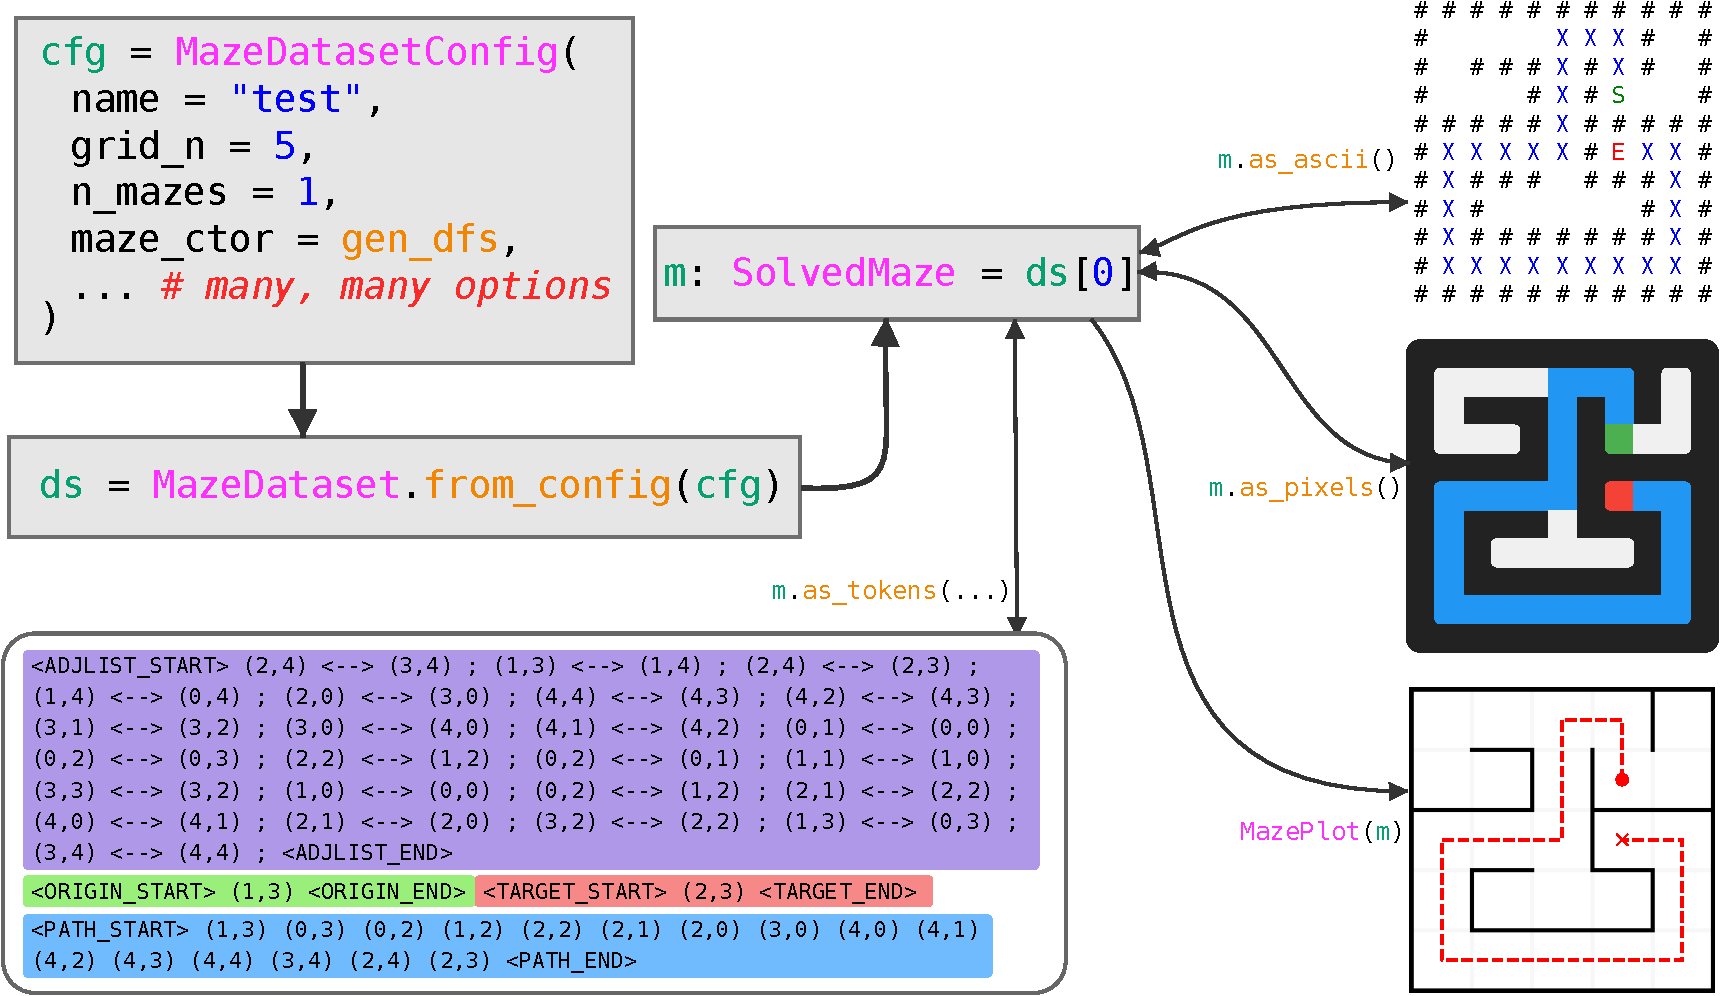
\includegraphics{docs/paper/diagram/diagram.pdf}%
};

\node[anchor=north west,
	hyperlink url={https://github.com},
	draw=blue, fill=blue!20, fill opacity=0.3,
	minimum width=2cm, minimum height=1cm]
	at ($(current page.north west)+(0,-1cm)$) {};

% Establish a coordinate system mapping the original SVG viewBox (1100x640)
% \begin{scope}[x={(img.south east)}, y={(img.north west)}]
	
% 	% 1. MazeDatasetConfig (for both "cfg" and "MazeDatasetConfig")
% 	\node[hyperlink url={https://understanding-search.github.io/maze-dataset/maze_dataset.html#MazeDatasetConfig},
% 			anchor=south west,
% 			draw=blue, fill=blue!20, fill opacity=0.3, line width=1pt,
% 			minimum width={(150-25)/1100*6in},
% 			minimum height={(60-30)/640*3.5in}]
% 		at ($(25/1100, {1 - 60/640})$) {};
	
% 	% 2. LatticeMazeGenerators.gen_dfs (the "gen_dfs" text)
% 	\node[hyperlink url={https://understanding-search.github.io/maze-dataset/maze_dataset.html#LatticeMazeGenerators.gen_dfs},
% 			anchor=south west,
% 			draw=blue, fill=blue!20, fill opacity=0.3, line width=1pt,
% 			minimum width={(150-45)/1100*6in},
% 			minimum height={(180-150)/640*3.5in}]
% 		at ($(45/1100, {1 - 180/640})$) {};
	
% 	% 3. MazeDataset (the "ds" and "MazeDataset" text)
% 	\node[hyperlink url={https://understanding-search.github.io/maze-dataset/maze_dataset.html#MazeDataset},
% 			anchor=south west,
% 			draw=blue, fill=blue!20, fill opacity=0.3, line width=1pt,
% 			minimum width={(150-25)/1100*6in},
% 			minimum height={(335-305)/640*3.5in}]
% 		at ($(25/1100, {1 - 335/640})$) {};
	
% 	% 4. MazeDataset.from_config (following MazeDataset on the same line)
% 	\node[hyperlink url={https://understanding-search.github.io/maze-dataset/maze_dataset.html#MazeDataset.from_config},
% 			anchor=south west,
% 			draw=blue, fill=blue!20, fill opacity=0.3, line width=1pt,
% 			minimum width={(300-150)/1100*6in},
% 			minimum height={(335-305)/640*3.5in}]
% 		at ($(150/1100, {1 - 335/640})$) {};
	
% 	% 5. SolvedMaze (the text starting at x≈424.6, y≈205)
% 	\node[hyperlink url={https://understanding-search.github.io/maze-dataset/maze_dataset.html#SolvedMaze},
% 			anchor=south west,
% 			draw=blue, fill=blue!20, fill opacity=0.3, line width=1pt,
% 			minimum width={(544.6-424.6)/1100*6in},  % 544.6 = 424.6+120
% 			minimum height={(205-165)/640*3.5in}]
% 		at ($(424.6/1100, {1 - 205/640})$) {};
	
% 	% 6. LatticeMaze.as_ascii (from x≈837.4, y≈125)
% 	\node[hyperlink url={https://understanding-search.github.io/maze-dataset/maze_dataset.html#LatticeMaze.as_ascii},
% 			anchor=south west,
% 			draw=blue, fill=blue!20, fill opacity=0.3, line width=1pt,
% 			minimum width={(937.4-837.4)/1100*6in},  % 937.4 = 837.4+100
% 			minimum height={(125-95)/640*3.5in}]
% 		at ($(837.4/1100, {1 - 125/640})$) {};
	
% 	% 7. LatticeMaze.as_pixels (from x≈836.1, y≈335)
% 	\node[hyperlink url={https://understanding-search.github.io/maze-dataset/maze_dataset.html#LatticeMaze.as_pixels},
% 			anchor=south west,
% 			draw=blue, fill=blue!20, fill opacity=0.3, line width=1pt,
% 			minimum width={(936.1-836.1)/1100*6in},  % 936.1 = 836.1+100
% 			minimum height={(335-305)/640*3.5in}]
% 		at ($(836.1/1100, {1 - 335/640})$) {};
	
% 	% 8. MazePlot (from x≈846.8, y≈555)
% 	\node[hyperlink url={https://understanding-search.github.io/maze-dataset/maze_dataset/plotting.html#MazePlot},
% 			anchor=south west,
% 			draw=blue, fill=blue!20, fill opacity=0.3, line width=1pt,
% 			minimum width={(966.8-846.8)/1100*6in},  % 966.8 = 846.8+120
% 			minimum height={(555-525)/640*3.5in}]
% 		at ($(846.8/1100, {1 - 555/640})$) {};
	
% 	% 9. LatticeMaze.as_tokens (from x≈571.1, y≈406)
% 	\node[hyperlink url={https://understanding-search.github.io/maze-dataset/maze_dataset.html#LatticeMaze.as_tokens},
% 			anchor=south west,
% 			draw=blue, fill=blue!20, fill opacity=0.3, line width=1pt,
% 			minimum width={(691.1-571.1)/1100*6in},  % 691.1 = 571.1+120
% 			minimum height={(406-376)/640*3.5in}]
% 		at ($(571.1/1100, {1 - 406/640})$) {};
	
% \end{scope}
\end{tikzpicture} 
  \end{minipage}
  \caption{Usage of maze-dataset. We create a `MazeDataset` from a `MazeDatasetConfig`. This contains `SolvedMaze` objects which can be converted to and from a variety of formats. Code in the image contains clickable links to \href{https://understanding-search.github.io/maze-dataset/maze_dataset.html}{documentation}. A variety of generated examples can be viewed \href{https://understanding-search.github.io/maze-dataset/examples/maze_examples.html}{here}.}
  \label{fig:diagram}
\end{figure}

\hypertarget{statement-of-need}{%
\section{Statement of Need}\label{statement-of-need}}

The generation of mazes with a given algorithm is not inherently a
complex task, but the ability to seamlessly switch out algorithms,
modify algorithm parameters, or filter by desired properties all while
preserving the ability to convert between different representations of
the maze is not trivial. This library aims to greatly streamline the
process of generating and working with datasets of mazes that can be
described as subgraphs of an \(n \times n\) lattice with boolean
connections and, optionally, start and end points that are nodes in the
graph. Furthermore, we place emphasis on a wide variety of possible text
output formats aimed at evaluating the spatial reasoning capabilities of
Large Language Models and other text-based transformer models.

For interpretability and behavioral research, algorithmic tasks offer
benefits by allowing systematic data generation and task decomposition,
as well as simplifying the process of circuit discovery
(\protect\hyperlink{ref-interpretability-survery}{Räuker et al., 2023}).
Although mazes are well suited for these investigations, we have found
that existing maze generation packages
(\protect\hyperlink{ref-cobbe2019procgen}{Cobbe et al., 2019};
\protect\hyperlink{ref-gh_Ehsan_2022}{Ehsan, 2022};
\protect\hyperlink{ref-harriesMazeExplorerCustomisable3D2019}{Harries et
al., n.d.}; \protect\hyperlink{ref-gh_Nemeth_2019}{Németh, 2019};
\protect\hyperlink{ref-easy_to_hard}{Schwarzschild, Borgnia, Gupta,
Bansal, et al., 2021}) do not support flexible maze generation
algorithms that provide fine-grained control of generation parameters
and the ability to easily transform between multiple representations of
the mazes (Images, Textual, Tokenized) for training and testing models.

\hypertarget{related-works}{%
\subsection{Related Works}\label{related-works}}

A multitude of public and open-source software packages exist for
generating mazes (\protect\hyperlink{ref-gh_Ehsan_2022}{Ehsan, 2022};
\protect\hyperlink{ref-gh_Nemeth_2019}{Németh, 2019};
\protect\hyperlink{ref-easy_to_hard}{Schwarzschild, Borgnia, Gupta,
Bansal, et al., 2021}). However, nearly all of these packages generate
and store mazes in a form that is not optimized for storage space or,
more importantly, computer readability. The mazes produces by other
packages are usually rasterized or in some form of image, rather than
the underlying graph structure, and this makes it difficult to work with
these datasets.

\begin{itemize}
\item
  Most prior works provide mazes in some kind of image or raster format,
  which is not suitable for training autoregressive text-based
  transformer models -- a key usage case this work seeks to enable.
  However, we still provide a variety of similar output formats:

  \begin{itemize}
  \tightlist
  \item
    we also include the \texttt{RasterizedMazeDataset} class, utilizing
    \texttt{as\_pixels()}, in our codebase, which can exactly mimic the
    outputs provided in
    \texttt{easy-to-hard-data}(\protect\hyperlink{ref-easy_to_hard}{Schwarzschild,
    Borgnia, Gupta, Bansal, et al., 2021}) and can be configured to be
    similar to the outputs of
    (\protect\hyperlink{ref-gh_Nemeth_2019}{Németh, 2019}).
  \item
    Our \texttt{as\_ascii()} method provides a format similar to that
    used in Oppenheim
    (\protect\hyperlink{ref-gh-oppenheimj2018maze}{2018}).
  \item
    Our \texttt{MazePlot} class provides a feature-rich plotting utility
    with support for multiple paths, heatmaps over positions, and more.
    This is similar to the outputs of Ehsan
    (\protect\hyperlink{ref-gh_Ehsan_2022}{2022})
  \end{itemize}
\item
  The text format provided by \texttt{SolvedMaze(...).as\_tokens()} is
  similar to that of (\protect\hyperlink{ref-eval-LLM-graphs}{Liu \& Wu,
  2023}), but provides over 5.8 million unique formats for converting
  mazes to a text stream. We maintain a single underlying format,
  meaning that the same maze can be turned into a variety of text
  streams to assess how the precise format of the text stream affects
  the model.
\item
  For rigorous investigations of the response of a model to various
  distributional shifts, preserving metadata about the generation
  algorithm with the dataset itself is essential. To this end, our
  package efficiently stores the dataset along with its metadata in a
  single human-readable file (\protect\hyperlink{ref-zanj}{M.
  Ivanitskiy, n.d.}). This metadata is loaded when the dataset is
  retrieved from disk and makes it simple to understand how exactly each
  maze was generated. As far as we are aware, no existing packages do
  this reliably.
\item
  Storing mazes as images is not only difficult to work with, but also
  inefficient. Directly storing adjacency matrices is also inefficient
  as subgraphs of the lattice are sparse. Storing adjacency lists can be
  efficient, but comes with a higher lookup cost and possible high
  comparison cost. We use a simple, efficient representation of mazes
  that is optimized for subgraphs of a \(d\)-dimensional finite lattice
  that we do not believe is used in any existing maze generation
  package.
\item
  Our package is easily installable with source code freely available.
  It is extensively tested, type hinted, benchmarked, and documented.
  Many other maze generation packages lack this level of rigor and
  scope, and some (\protect\hyperlink{ref-ayaz2008maze}{Ayaz et al.,
  2008}) appear to simply no longer be accessible.
\end{itemize}

\hypertarget{features}{%
\section{Features}\label{features}}

\hypertarget{generation}{%
\subsection{Generation and Usage}\label{generation}}

Our package can be installed from
\href{https://pypi.org/project/maze-dataset/}{PyPi} via
\texttt{pip\ install\ maze-dataset}, or directly from the
\href{https://github.com/understanding-search/maze-dataset}{git
repository} (\protect\hyperlink{ref-maze-dataset-github}{Michael I.
Ivanitskiy et al., 2023a}).

To create a dataset, we first create a \texttt{MazeDatasetConfig}
configuration object, which specifies the seed, number, and size of
mazes, as well as the generation algorithm and its corresponding
parameters. This object is passed to a \texttt{MazeDataset} class to
create a dataset. Crucially, this \texttt{MazeDataset} mimics the
interface of a PyTorch (\protect\hyperlink{ref-pytorch}{Paszke et al.,
2019}) \texttt{Dataset}, and can thus be easily incorporated into
existing data pre-processing and training pipelines, e.g., through the
use of a \texttt{Dataloader} class.

\begin{Shaded}
\begin{Highlighting}[]
\ImportTok{from}\NormalTok{ maze\_dataset }\ImportTok{import}\NormalTok{ MazeDataset, MazeDatasetConfig, LatticeMazeGenerators}
\NormalTok{cfg: MazeDatasetConfig }\OperatorTok{=}\NormalTok{ MazeDatasetConfig(}
\NormalTok{    name}\OperatorTok{=}\StringTok{"example"}\NormalTok{, }
\NormalTok{    grid\_n}\OperatorTok{=}\DecValTok{3}\NormalTok{, }
\NormalTok{    n\_mazes}\OperatorTok{=}\DecValTok{32}\NormalTok{, }
\NormalTok{    maze\_ctor}\OperatorTok{=}\NormalTok{LatticeMazeGenerators.gen\_dfs,}
\NormalTok{)}
\NormalTok{dataset: MazeDataset }\OperatorTok{=}\NormalTok{ MazeDataset.from\_config(cfg)}
\end{Highlighting}
\end{Shaded}

When initializing mazes, further configuration options can be specified
through the \texttt{from\_config()} factory method as necessary. Options
allow for saving/loading existing datasets instead of regenerating, and
parallelization options for generation. Available maze generation
algorithms are static methods of the \texttt{LatticeMazeGenerators}
class and include the following:

\begin{itemize}
\tightlist
\item
  \texttt{gen\_dfs} \textbf{(randomized depth-first search)}: Parameters
  can be passed to constrain the number of accessible cells, the number
  of forks in the maze, and the maximum tree depth. Creates a spanning
  tree by default or a partially spanning tree if constrained.
\item
  \texttt{gen\_wilson} \textbf{(Wilson's algorithm)}: Generates a random
  spanning tree via loop-erased random walk
  (\protect\hyperlink{ref-wilson}{Wilson, 1996}).
\item
  \texttt{gen\_percolation} \textbf{(percolation)}: Starting with no
  connections, every possible lattice connection is set to either true
  or false with some probability \(p\), independently of all other
  connections. For the kinds of graphs that this process generates, we
  refer to existing work
  (\protect\hyperlink{ref-percolation}{Duminil-Copin, 2017};
  \protect\hyperlink{ref-percolation-clustersize}{Fisher \& Essam,
  2004}).
\item
  \texttt{gen\_dfs\_percolation} \textbf{(randomized depth-first search
  with percolation)}: A connection exists if it exists in a maze
  generated via \texttt{gen\_dfs\ OR\ gen\_percolation}. Useful for
  generating mazes that are not acyclic graphs.
\end{itemize}

Furthermore, a dataset of mazes can be filtered to satisfy certain
properties:

\begin{Shaded}
\begin{Highlighting}[]
\NormalTok{dataset\_filtered: MazeDataset }\OperatorTok{=}\NormalTok{ dataset.filter\_by.path\_length(min\_length}\OperatorTok{=}\DecValTok{3}\NormalTok{)}
\end{Highlighting}
\end{Shaded}

Custom filters can be specified, and several filters are included:

\begin{itemize}
\tightlist
\item
  \texttt{path\_length(min\_length:\ int)}: shortest length from the
  origin to target should be at least \texttt{min\_length}.
\item
  \texttt{start\_end\_distance(min\_distance:\ int)}: Manhattan distance
  between start and end should be at least \texttt{min\_distance},
  ignoring walls.
\item
  \texttt{remove\_duplicates(...)}: remove mazes which are similar to
  others in the dataset, measured via Hamming distance.
\item
  \texttt{remove\_duplicates\_fast()}: remove mazes which are exactly
  identical to others in the dataset.
\end{itemize}

All implemented maze generation algorithms are stochastic by nature. For
reproducibility, the \texttt{seed} parameter of
\texttt{MazeDatasetConfig} may be set. In practice, we do not find that
exact duplicates of mazes are generated with any meaningful frequency,
even when generating large datasets.

\hypertarget{visual-output-formats}{%
\section{Visual Output Formats}\label{visual-output-formats}}

Internally, mazes are \texttt{SolvedMaze} objects, which have path
information, and a connection list optimized for storing sub-graphs of a
lattice. These objects can be converted to and from several formats.

\begin{longtable}[]{@{}
  >{\raggedright\arraybackslash}p{(\columnwidth - 4\tabcolsep) * \real{0.3250}}
  >{\raggedright\arraybackslash}p{(\columnwidth - 4\tabcolsep) * \real{0.3500}}
  >{\raggedright\arraybackslash}p{(\columnwidth - 4\tabcolsep) * \real{0.3250}}@{}}
\toprule\noalign{}
\begin{minipage}[b]{\linewidth}\raggedright
\texttt{as\_ascii()}
\end{minipage} & \begin{minipage}[b]{\linewidth}\raggedright
\texttt{as\_pixels()}
\end{minipage} & \begin{minipage}[b]{\linewidth}\raggedright
\texttt{MazePlot()}
\end{minipage} \\
\midrule\noalign{}
\endhead
\bottomrule\noalign{}
\endlastfoot
Simple text format for displaying mazes, useful for debugging in a
terminal environment. & \texttt{numpy} array of \texttt{dtype=uint8} and
shape \texttt{(height,\ width,\ 3)}. The last dimension is RGB color. &
feature-rich plotting utility with support for multiple paths, heatmaps
over positions, and more. \\
\end{longtable}

\begin{figure}
\hypertarget{fig:visualoutputs}{%
\centering
\includegraphics{docs/paper/figures/output-fmts.pdf}
\caption{Various output formats. Top row (left to right): ASCII diagram,
rasterized pixel grid, and advanced display.}\label{fig:visualoutputs}
}
\end{figure}

\hypertarget{training}{%
\subsection{Visual Outputs for Training and Evaluation}\label{training}}

In previous work, maze tasks have been used with Recurrent Convolutional
Neural Network (RCNN) derived architectures
(\protect\hyperlink{ref-deepthinking}{Schwarzschild, Borgnia, Gupta,
Huang, et al., 2021}). To facilitate the use of our package in this
context, we replicate the format of
(\protect\hyperlink{ref-easy_to_hard}{Schwarzschild, Borgnia, Gupta,
Bansal, et al., 2021}) and provide the \texttt{RasterizedMazeDataset}
class which returns rasterized pairs of (input, target) mazes as shown
in \autoref{fig:e2hraster} below.

\begin{figure}
\hypertarget{fig:e2hraster}{%
\centering

\includegraphics[width=0.3\textwidth,height=\textheight]{docs/paper/figures/maze-raster-input-target.pdf}
\caption{Input is the rasterized maze without the path marked (left),
and provide as a target the maze with all but the correct path removed.
Configuration options exist to adjust whether endpoints are included and
if empty cells should be filled in.}\label{fig:e2hraster}
}
\end{figure}

\hypertarget{tokenized-output-formats}{%
\section{Tokenized Output Formats}\label{tokenized-output-formats}}

To train autoregressive text models such as transformers, we convert
mazes to token sequences in two steps. First, the maze is stringified
using \texttt{as\_tokens()}. The \texttt{MazeTokenizerModular} class
provides a powerful interface for configuring maze stringification
behavior. Second, the sequence of strings is tokenized into integers
using \texttt{encode()}. Tokenization uses a fixed vocabulary for
simplicity. Mazes up to 50x50 are supported using unique tokens, and up
to 128x128 when using coordinate tuple tokens.

\hypertarget{mtm}{%
\subsection{\texorpdfstring{Stringification Options and
\texttt{MazeTokenizerModular}}{Stringification Options and MazeTokenizerModular}}\label{mtm}}

There are many algorithms by which one might tokenize a 2D maze into a
1D format usable by autoregressive text models. Training multiple models
on the encodings output from each of these algorithms may produce very
different internal representations, learned solution algorithms, and
levels of performance. To explore how different maze tokenization
algorithms affect these models, the \texttt{MazeTokenizerModular} class
contains a rich set of options to customize how mazes are stringified.
This class contains 19 discrete parameters, resulting in 5.9 million
unique tokenizers. But wait, there's more! There are 6 additional
parameters available in the library which are untested but further
expand the the number of tokenizers by a factor of \(44/3\) to 86
million.

All output sequences consist of four token regions representing
different features of the maze. These regions are distinguished by color
in Figure below.

\begin{itemize}
\tightlist
\item
  {Adjacency list}: A text representation of the lattice graph
\item
  {Origin}: Starting coordinate
\item
  {Target}: Ending coordinate
\item
  {Path}: Maze solution sequence from the start to the end
\end{itemize}

\begin{figure}
\centering
\includegraphics{docs/paper/figures/outputs-tokens-colored.tex}
\caption{Example text output format with token regions highlighted.}
\end{figure}

Each \texttt{MazeTokenizerModular} is constructed from a set of several
\texttt{\_TokenizerElement} objects, each of which specifies how
different token regions or other elements of the stringification are
produced.

\begin{figure}
\centering
\includegraphics{docs/paper/figures/TokenizerElement_structure.pdf}
\caption{Nested internal structure of \texttt{\_TokenizerElement}
objects inside a typical \texttt{MazeTokenizerModular} object.}
\end{figure}

Optional delimiter tokens may be added in many places in the output.
Delimiter options are all configured using the parameters named
\texttt{pre}, \texttt{intra}, and \texttt{post} in various
\texttt{\_TokenizerElement} classes. Each option controls a unique
delimiter token. Here we describe each \texttt{\_TokenizerElement} and
the behaviors they support. We also discuss some of the model behaviors
and properties that may be investigated using these options.

\hypertarget{coordtokenizer}{%
\subsubsection{Coordinates}\label{coordtokenizer}}

The \texttt{\_CoordTokenizer} object controls how coordinates in the
lattice are represented in across all token regions. Options include:

\begin{itemize}
\tightlist
\item
  \textbf{Unique tokens}: Each coordinate is represented as a single
  unique token \texttt{"(i,j)"}
\item
  \textbf{Coordinate tuple tokens}: Each coordinate is represented as a
  sequence of 2 tokens, respectively encoding the row and column
  positions: \texttt{{[}"i",\ ",",\ "j"{]}}
\end{itemize}

\hypertarget{adjlisttokenizer}{%
\subsubsection{Adjacency List}\label{adjlisttokenizer}}

The \texttt{\_AdjListTokenizer} object controls this token region. All
tokenizations represent the maze connectivity as a sequence of
connections or walls between pairs of adjacent coordinates in the
lattice.

\begin{itemize}
\tightlist
\item
  \texttt{\_EdgeSubset}: Specifies the subset of lattice edges to be
  tokenized

  \begin{itemize}
  \tightlist
  \item
    \textbf{All edges}: Every edge in the lattice
  \item
    \textbf{Connections}: Only edges which contain a connection
  \item
    \textbf{Walls}: Only edges which contain a wall
  \end{itemize}
\item
  \texttt{\_EdgePermuter}: Specifies how to sequence the two coordinates
  in each lattice edge

  \begin{itemize}
  \tightlist
  \item
    \textbf{Random}
  \item
    \textbf{Sorted}: The smaller coordinate always comes first
  \item
    \textbf{Both permutations}: Each edge is represented twice, once
    with each permutation. This option attempts to represent connections
    in a more directionally symmetric manner. Including only one
    permutation of each edge may affect models' internal representations
    of edges, treating a path traversing the edge differently depending
    on if the coordinate sequence in the path matches the sequence in
    the adjacency list.
  \end{itemize}
\item
  \texttt{shuffle\_d0}: Whether to shuffle the edges randomly or sort
  them in the output by their first coordinate
\item
  \texttt{connection\_token\_ordinal}: Location in the sequence of the
  token representing whether the edge is a connection or a wall
\end{itemize}

\hypertarget{pathtokenizer}{%
\subsubsection{Path}\label{pathtokenizer}}

The \texttt{\_PathTokenizer} object controls this token region. Paths
are all represented as a sequence of steps moving from the start to the
end position.

\begin{itemize}
\tightlist
\item
  \texttt{\_StepSize}: Specifies the size of each step

  \begin{itemize}
  \tightlist
  \item
    \textbf{Singles}: Every coordinate traversed between start and end
    is directly represented
  \item
    \textbf{Forks}: Only coordinates at forking points in the maze are
    represented. The paths between forking points are implicit. Using
    this option might train models more directly to represent forking
    points differently from coordinates where the maze connectivity
    implies an obvious next step in the path.
  \end{itemize}
\item
  \texttt{\_StepTokenizer}: Specifies how an individual step is
  represented

  \begin{itemize}
  \tightlist
  \item
    \textbf{Coordinate}: The coordinates of each step are directly
    tokenized using a \texttt{\_CoordTokenizer}
  \item
    \textbf{Cardinal direction}: A single token corresponding to the
    cardinal direction taken at the starting position of that step.
    E.g., \texttt{NORTH}, \texttt{SOUTH}. If using a \texttt{\_StepSize}
    other than \textbf{Singles}, this direction may not correspond to
    the final direction traveled to arrive at the end position of the
    step.
  \item
    \textbf{Relative direction}: A single token corresponding to the
    first-person perspective relative direction taken at the starting
    position of that step. E.g., \texttt{RIGHT}, \texttt{LEFT}.
  \item
    \textbf{Distance}: A single token corresponding to the number of
    coordinate positions traversed in that step. E.g., using a
    \texttt{\_StepSize} of \textbf{Singles}, the \textbf{Distance} token
    would be the same for each step, corresponding to a distance of 1
    coordinate. This option is only of interest in combination with a
    \texttt{\_StepSize} other than \textbf{Singles}.
  \end{itemize}
\end{itemize}

A \texttt{\_PathTokenizer} contains a sequence of one or more unique
\texttt{\_StepTokenizer} objects. Different step representations may be
mixed and permuted, allowing for investigation of model representations
of multiple aspects of a maze solution at once.

\hypertarget{token-training}{%
\subsection{Tokenized Outputs for Training and
Evaluation}\label{token-training}}

During deployment we provide only the prompt up to the
\texttt{\textless{}PATH\_START\textgreater{}} token.

Examples of usage of this dataset to train autoregressive transformers
can be found in our \texttt{maze-transformer} library
(\protect\hyperlink{ref-maze-transformer-github}{Michael I. Ivanitskiy
et al., 2023b}). Other tokenization and vocabulary schemes are also
included, such as representing each coordinate as a pair of \(i,j\)
index tokens.

\hypertarget{extensibility}{%
\subsection{Extensibility}\label{extensibility}}

The tokenizer architecture is purposefully designed such that adding and
testing a wide variety of new tokenization algorithms is fast and
minimizes disturbances to functioning code. This is enabled by the
modular architecture and the automatic inclusion of any new tokenizers
in integration tests. To create a new tokenizer, developers forking the
library may simply create their own \texttt{\_TokenizerElement} subclass
and implement the abstract methods. If the behavior change is
sufficiently small, simply adding a parameter to an existing
\texttt{\_TokenizerElement} subclass and updating its implementation
will suffice. For small additions, simply adding new cases to existing
unit tests will suffice.

The breadth of tokenizers is also easily scaled in the opposite
direction. Due to the exponential scaling of parameter combinations,
adding a small number of new features can significantly slow certain
procedures which rely on constructing all possible tokenizers, such as
integration tests. If any existing subclass contains features which
aren't needed, a developer tool decorator is provided which can be
applied to the unneeded \texttt{\_TokenizerElement} subclasses to prune
those features and compact the available space of tokenizers.

\hypertarget{benchmarks}{%
\section{Benchmarks of Generation Speed}\label{benchmarks}}

We provide approximate benchmarks for relative generation time across
various algorithms, parameter choices, maze sizes, and dataset sizes.

\begin{longtable}[]{@{}
  >{\raggedright\arraybackslash}p{(\columnwidth - 10\tabcolsep) * \real{0.1680}}
  >{\raggedright\arraybackslash}p{(\columnwidth - 10\tabcolsep) * \real{0.2080}}
  >{\raggedright\arraybackslash}p{(\columnwidth - 10\tabcolsep) * \real{0.1360}}
  >{\raggedright\arraybackslash}p{(\columnwidth - 10\tabcolsep) * \real{0.1520}}
  >{\raggedright\arraybackslash}p{(\columnwidth - 10\tabcolsep) * \real{0.2000}}
  >{\raggedright\arraybackslash}p{(\columnwidth - 10\tabcolsep) * \real{0.1360}}@{}}
\toprule\noalign{}
\begin{minipage}[b]{\linewidth}\raggedright
Method \& Parameters
\end{minipage} & \begin{minipage}[b]{\linewidth}\raggedright
Average time per maze (ms)
\end{minipage} & \begin{minipage}[b]{\linewidth}\raggedright
\end{minipage} & \begin{minipage}[b]{\linewidth}\raggedright
\end{minipage} & \begin{minipage}[b]{\linewidth}\raggedright
\end{minipage} & \begin{minipage}[b]{\linewidth}\raggedright
\end{minipage} \\
\midrule\noalign{}
\endhead
\bottomrule\noalign{}
\endlastfoot
Generation algorithm & Generation parameters & all sizes & small
(\(g \leq 10\)) & medium (\(10 < g \leq 32\)) & large (\(g > 32\)) \\
:===============: & :===============: & :===============: &
:===============: & :===============: & :===============: \\
gen\_dfs & accessible\_cells=20 & 2.4 & 2.4 & 2.6 & 2.4 \\
gen\_dfs & do\_forks=False & 3.0 & 2.4 & 3.7 & 3.8 \\
gen\_dfs & max\_tree\_depth=0.5 & 4.5 & 2.2 & 4.9 & 11.6 \\
gen\_dfs & -- & 31.1 & 2.8 & 28.0 & 136.5 \\
gen\_dfs\_percolation & p=0.1 & 53.9 & 3.6 & 42.5 & 252.9 \\
gen\_dfs\_percolation & p=0.4 & 58.8 & 3.7 & 44.7 & 280.2 \\
gen\_percolation & -- & 59.1 & 3.3 & 43.6 & 285.2 \\
gen\_wilson & -- & 767.9 & 10.1 & 212.9 & 4530.4 \\
:===============: & :===============: & :===============: &
:===============: & :===============: & :===============: \\
\textbf{median (all runs)} & & 10.8 & 6.0 & 44.4 & 367.7 \\
\textbf{mean (all runs)} & & 490.0 & 11.7 & 187.2 & 2769.6 \\
\end{longtable}

\begin{figure}
\centering
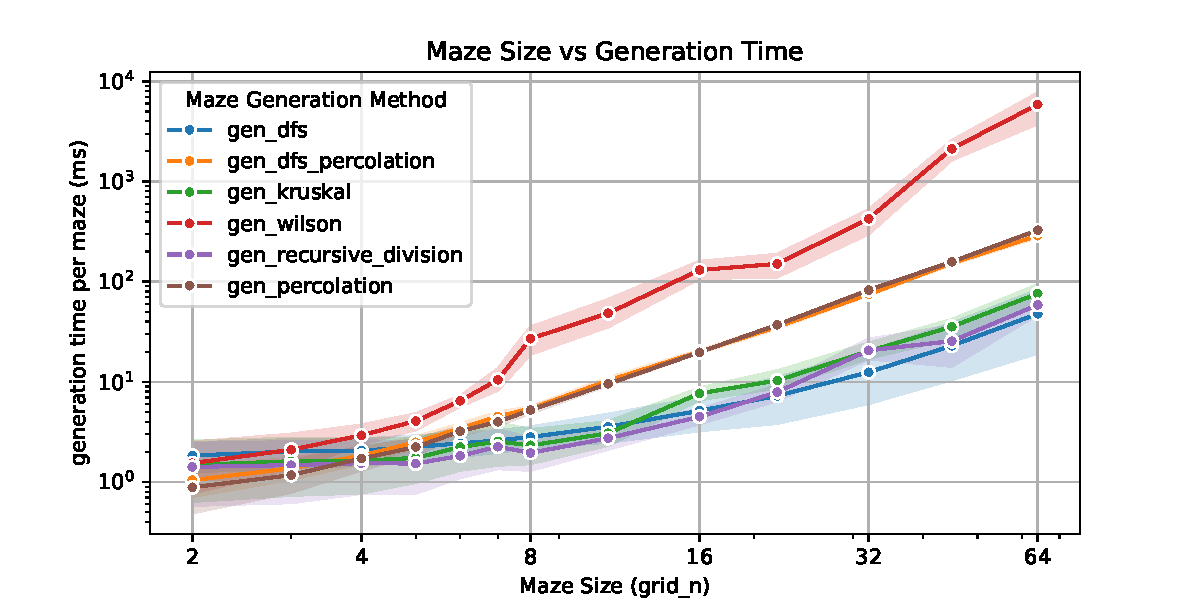
\includegraphics[width=0.95\textwidth,height=\textheight]{docs/paper/figures/gridsize-vs-gentime.pdf}
\caption{Plots of maze generation time. Generation time scales
exponentially with maze size for all algorithms (left). Generation time
does not depend on the number of mazes being generated, and there is
minimal overhead to initializing the generation process for a small
dataset (right). Wilson's algorithm is notably less efficient than
others and has high variance. Note that for both plots, values are
averaged across all parameter sets for that algorithm, and
parallelization is disabled.}
\end{figure}

\hypertarget{implementation}{%
\section{Implementation}\label{implementation}}

We refer to our GitHub repository
(\protect\hyperlink{ref-maze-dataset-github}{Michael I. Ivanitskiy et
al., 2023a}) for documentation and up-to-date implementation details.

This package utilizes a simple, efficient representation of mazes. Using
an adjacency list to represent mazes would lead to a poor lookup time of
whether any given connection exists, whilst using a dense adjacency
matrix would waste memory by failing to exploit the structure (e.g.,
only 4 of the diagonals would be filled in). Instead, we describe mazes
with the following simple representation: for a \(d\)-dimensional
lattice with \(r\) rows and \(c\) columns, we initialize a boolean array
\(A = \{0, 1\}^{d \times r \times c}\), which we refer to in the code as
a \texttt{connection\_list}. The value at \(A[0,i,j]\) determines
whether a downward connection exists from node \([i,j]\) to
\([i+1, j]\). Likewise, the value at \(A[1,i,j]\) determines whether a
rightwards connection to \([i, j+1]\) exists. Thus, we avoid duplication
of data about the existence of connections, at the cost of requiring
additional care with indexing when looking for a connection upwards or
to the left. Note that this setup allows for a periodic lattice.

To produce solutions to mazes, two points are selected uniformly at
random without replacement from the connected component of the maze, and
the \(A^*\) algorithm (\protect\hyperlink{ref-A_star}{Hart et al.,
1968}) is applied to find the shortest path between them.

Parallelization is implemented via the \texttt{multiprocessing} module
in the Python standard library, and parallel generation can be
controlled via keyword arguments to the
\texttt{MazeDataset.from\_config()} function.

\hypertarget{limitations}{%
\subsection{\texorpdfstring{Limitations of
\texttt{maze-dataset}}{Limitations of maze-dataset}}\label{limitations}}

For simplicity, the package primarily supports mazes that are sub-graphs
of a 2-dimensional rectangular lattice. Some support for
higher-dimensional lattices is present, but not all output formats are
adapted for higher dimensional mazes.
\protect\hyperlink{implementation-implementation}{Implementation}
\protect\hyperlink{implementation-implementation}{Implementation}

\hypertarget{usage-in-research}{%
\section{Usage in Research}\label{usage-in-research}}

This package was originally built for the needs of the
(\protect\hyperlink{ref-maze-transformer-github}{Michael I. Ivanitskiy
et al., 2023b}) project, which aims to investigate spatial planning and
world models in autoregressive transformer models trained on mazes Spies
et al. (\protect\hyperlink{ref-spies2024causalworldmodels}{2024}). This
project has also adapted itself to be useful for work on understanding
the mechanisms by which recurrent convolutional and implicit networks
(\protect\hyperlink{ref-fung2022jfb}{Fung et al., 2022}) solve mazes
given a rasterized view
(\protect\hyperlink{ref-knutson2024logicalextrapolation}{Knutson et al.,
2024}), and for this we match the output format of
(\protect\hyperlink{ref-easy_to_hard}{Schwarzschild, Borgnia, Gupta,
Bansal, et al., 2021}).

This package has also been utilized in work by other groups:

\begin{itemize}
\item
  (\protect\hyperlink{ref-nolte2024multistep}{Nolte et al., 2024}) use
  \texttt{maze-dataset} to compare the effectiveness of transformers
  trained with the MLM-\(\mathcal{U}\)
  (\protect\hyperlink{ref-MLMU-kitouni2024factorization}{Kitouni et al.,
  2024}) multistep prediction objective against standard autoregressive
  training for multi-step planning on our maze task.
\item
  (\protect\hyperlink{ref-wang2024imperative}{Wang et al., 2024}) and
  (\protect\hyperlink{ref-chen2024iaimperative}{Chen et al., 2024}) use
  \texttt{maze-dataset} to study the effectiveness of imperative
  learning
\end{itemize}

\hypertarget{conclusion}{%
\section{Conclusion}\label{conclusion}}

The
\href{https://github.com/understanding-search/maze-dataset}{\texttt{maze-dataset}}
library (\protect\hyperlink{ref-maze-dataset-github}{Michael I.
Ivanitskiy et al., 2023a}) introduced in this paper provides a flexible
and extensible toolkit for generating, processing, and analyzing maze
datasets. By supporting various procedural generation algorithms and
conversion utilities, it enables the creation of mazes with customizable
properties to suit diverse research needs. Planned improvements to the
\texttt{maze-dataset} include adding more generation algorithms (such as
Prim's algorithm (\protect\hyperlink{ref-dijkstra-prim}{Dijkstra, 1959};
\protect\hyperlink{ref-jarnik-prim}{Jarnık, 1930};
\protect\hyperlink{ref-prim}{Prim, 1957}) and Kruskal's algorithm
(\protect\hyperlink{ref-kruskal}{Kruskal, 1956}), among others
(\protect\hyperlink{ref-mazegen_analysis}{Gabrovšek, 2019})), adding the
ability to augment a maze with an adjacency list to add ``shortcuts'' to
the maze, and resolving certain limitations detailed in Section
\protect\hyperlink{limitations}{Limitations}.

\hypertarget{acknowledgements}{%
\section{Acknowledgements}\label{acknowledgements}}

This work was partially supported by and many of the authors were
brought together by AI Safety Camp and AI Safety Support. This work was
partially funded by National Science Foundation awards DMS-2110745 and
DMS-2309810. We are also grateful to LTFF and FAR Labs for hosting three
of the authors for a Residency Visit, and to various members of FAR's
technical staff for their advice. We thank the Mines Optimization and
Deep Learning group (MODL) for fruitful discussions. We also thank
Michael Rosenberg for recommending the usage of Finite State Transducers
for storing tokenizer validation information.

\hypertarget{references}{%
\section*{References}\label{references}}
\addcontentsline{toc}{section}{References}

\hypertarget{refs}{}
\begin{CSLReferences}{1}{0.5}
\leavevmode\vadjust pre{\hypertarget{ref-mazegenerator-net}{}}%
Alance AB. (2019). \emph{Maze generator}.
\url{http://www.mazegenerator.net}.

\leavevmode\vadjust pre{\hypertarget{ref-ayaz2008maze}{}}%
Ayaz, H., Allen, S. L., Platek, S. M., \& Onaral, B. (2008). Maze suite
1.0: A complete set of tools to prepare, present, and analyze
navigational and spatial cognitive neuroscience experiments.
\emph{Behavior Research Methods}, \emph{40}, 353--359.

\leavevmode\vadjust pre{\hypertarget{ref-chen2024iaimperative}{}}%
Chen, X., Yang, F., \& Wang, C. (2024). iA \(\^{}*\): Imperative
learning-based a \(\^{}*\) search for pathfinding. \emph{arXiv Preprint
arXiv:2403.15870}.

\leavevmode\vadjust pre{\hypertarget{ref-cobbe2019procgen}{}}%
Cobbe, K., Hesse, C., Hilton, J., \& Schulman, J. (2019). Leveraging
procedural generation to benchmark reinforcement learning. \emph{arXiv
Preprint arXiv:1912.01588}.

\leavevmode\vadjust pre{\hypertarget{ref-dijkstra-prim}{}}%
Dijkstra, E. W. (1959). \emph{A note on two problems in connexion with
graphs:({Numerische Mathematik}, 1 (1959), p 269-271)}.

\leavevmode\vadjust pre{\hypertarget{ref-percolation}{}}%
Duminil-Copin, H. (2017). \emph{Sixty years of percolation} (No.
arXiv:1712.04651). {arXiv}. \url{http://arxiv.org/abs/1712.04651}

\leavevmode\vadjust pre{\hypertarget{ref-gh_Ehsan_2022}{}}%
Ehsan, E. (2022). \emph{Maze}. \url{https://github.com/emadehsan/maze}

\leavevmode\vadjust pre{\hypertarget{ref-percolation-clustersize}{}}%
Fisher, M. E., \& Essam, J. W. (2004). Some {Cluster Size} and
{Percolation Problems}. \emph{Journal of Mathematical Physics},
\emph{2}(4), 609--619. \url{https://doi.org/10.1063/1.1703745}

\leavevmode\vadjust pre{\hypertarget{ref-fung2022jfb}{}}%
Fung, S. W., Heaton, H., Li, Q., McKenzie, D., Osher, S., \& Yin, W.
(2022). Jfb: Jacobian-free backpropagation for implicit networks.
\emph{Proceedings of the AAAI Conference on Artificial Intelligence},
\emph{36}, 6648--6656.

\leavevmode\vadjust pre{\hypertarget{ref-mazegen_analysis}{}}%
Gabrovšek. (2019). Analysis of maze generating algorithms. \emph{{IPSI
Transactions} on {Internet Research}}, \emph{15.1}, 23--30.
\url{http://www.ipsitransactions.org/journals/papers/tir/2019jan/p5.pdf}

\leavevmode\vadjust pre{\hypertarget{ref-mathematica-maze}{}}%
Guo, C., Barthelet, L., \& Morris, R. (2011). \emph{Maze generator and
solver}. Wolfram Demonstrations Project,
\url{https://demonstrations.wolfram.com/MazeGeneratorAndSolver/}.

\leavevmode\vadjust pre{\hypertarget{ref-harriesMazeExplorerCustomisable3D2019}{}}%
Harries, L., Lee, S., Rzepecki, J., Hofmann, K., \& Devlin, S. (n.d.).
{MazeExplorer}: {A Customisable 3D Benchmark} for {Assessing
Generalisation} in {Reinforcement Learning}. \emph{2019 {IEEE Conf}.
{Games CoG}}, 1--4.

\leavevmode\vadjust pre{\hypertarget{ref-A_star}{}}%
Hart, P. E., Nilsson, N. J., \& Raphael, B. (1968). A {Formal Basis} for
the {Heuristic Determination} of {Minimum Cost Paths}. \emph{IEEE
Transactions on Systems Science and Cybernetics}, \emph{4}(2), 100--107.
\url{https://doi.org/10.1109/TSSC.1968.300136}

\leavevmode\vadjust pre{\hypertarget{ref-zanj}{}}%
Ivanitskiy, M. (n.d.). \emph{ZANJ}.
\url{https://github.com/mivanit/ZANJ}

\leavevmode\vadjust pre{\hypertarget{ref-maze-dataset-github}{}}%
Ivanitskiy, Michael I., Shah, R., Spies, A. F., Räuker, T., Valentine,
D., Rager, C., Quirke, L., Corlouer, G., \& Mathwin, C. (2023a).
\emph{Maze dataset}.
\url{https://github.com/understanding-search/maze-dataset}

\leavevmode\vadjust pre{\hypertarget{ref-maze-transformer-github}{}}%
Ivanitskiy, Michael I., Shah, R., Spies, A. F., Räuker, T., Valentine,
D., Rager, C., Quirke, L., Corlouer, G., \& Mathwin, C. (2023b).
\emph{Maze transformer interpretability}.
\url{https://github.com/understanding-search/maze-transformer}

\leavevmode\vadjust pre{\hypertarget{ref-ivanitskiy2023structuredworldreps}{}}%
Ivanitskiy, Michael Igorevich, Spies, A. F., Räuker, T., Corlouer, G.,
Mathwin, C., Quirke, L., Rager, C., Shah, R., Valentine, D., Behn, C.
D., \& others. (2023). Structured world representations in maze-solving
transformers. \emph{arXiv Preprint arXiv:2312.02566}.

\leavevmode\vadjust pre{\hypertarget{ref-jarnik-prim}{}}%
Jarnık, V. (1930). About a certain minimal problem. \emph{Práce Moravské
Prırodovedecké Spolecnosti}, \emph{6}, 57--63.

\leavevmode\vadjust pre{\hypertarget{ref-MLMU-kitouni2024factorization}{}}%
Kitouni, O., Nolte, N. S., Williams, A., Rabbat, M., Bouchacourt, D., \&
Ibrahim, M. (2024). The factorization curse: Which tokens you predict
underlie the reversal curse and more. \emph{Advances in Neural
Information Processing Systems}, \emph{37}, 112329--112355.

\leavevmode\vadjust pre{\hypertarget{ref-knutson2024logicalextrapolation}{}}%
Knutson, B., Rabeendran, A. C., Ivanitskiy, M., Pettyjohn, J.,
Diniz-Behn, C., Fung, S. W., \& McKenzie, D. (2024). On logical
extrapolation for mazes with recurrent and implicit networks.
\emph{arXiv Preprint arXiv:2410.03020}.

\leavevmode\vadjust pre{\hypertarget{ref-kruskal}{}}%
Kruskal, J. B. (1956). On the shortest spanning subtree of a graph and
the traveling salesman problem. \emph{Proceedings of the American
Mathematical Society}, \emph{7}(1), 48--50.
\url{https://doi.org/10.1090/S0002-9939-1956-0078686-7}

\leavevmode\vadjust pre{\hypertarget{ref-eval-LLM-graphs}{}}%
Liu, C., \& Wu, B. (2023). Evaluating large language models on graphs:
Performance insights and comparative analysis. \emph{arXiv Preprint
arXiv:2308.11224}.

\leavevmode\vadjust pre{\hypertarget{ref-mdl-suite}{}}%
Nag, A. (2020). MDL suite: A language, generator and compiler for
describing mazes. \emph{Journal of Open Source Software}, \emph{5}(46),
1815.

\leavevmode\vadjust pre{\hypertarget{ref-gh_Nemeth_2019}{}}%
Németh, F. (2019). \emph{Maze-generation-algorithms}.
\url{https://github.com/ferenc-nemeth/maze-generation-algorithms}

\leavevmode\vadjust pre{\hypertarget{ref-nolte2024multistep}{}}%
Nolte, N., Kitouni, O., Williams, A., Rabbat, M., \& Ibrahim, M. (2024).
Transformers can navigate mazes with multi-step prediction. \emph{arXiv
Preprint arXiv:2412.05117}.

\leavevmode\vadjust pre{\hypertarget{ref-gh-oppenheimj2018maze}{}}%
Oppenheim, J. (2018). \emph{Maze-generator: Generate a random maze
represented as a 2D array using depth-first search}.
\url{https://github.com/oppenheimj/maze-generator/}; GitHub.

\leavevmode\vadjust pre{\hypertarget{ref-pytorch}{}}%
Paszke, A., Gross, S., Massa, F., Lerer, A., Bradbury, J., Chanan, G.,
Killeen, T., Lin, Z., Gimelshein, N., Antiga, L., Desmaison, A., Kopf,
A., Yang, E., DeVito, Z., Raison, M., Tejani, A., Chilamkurthy, S.,
Steiner, B., Fang, L., \ldots{} Chintala, S. (2019). {PyTorch: An
Imperative Style, High-Performance Deep Learning Library}. In H.
Wallach, H. Larochelle, A. Beygelzimer, F. d'Alché-Buc, E. Fox, \& R.
Garnett (Eds.), \emph{Advances in neural information processing systems
32} (pp. 8024--8035). Curran Associates, Inc.
\url{http://papers.neurips.cc/paper/9015-pytorch-an-imperative-style-high-performance-deep-learning-library.pdf}

\leavevmode\vadjust pre{\hypertarget{ref-prim}{}}%
Prim, R. C. (1957). Shortest connection networks and some
generalizations. \emph{The Bell System Technical Journal}, \emph{36}(6),
1389--1401.

\leavevmode\vadjust pre{\hypertarget{ref-interpretability-survery}{}}%
Räuker, T., Ho, A., Casper, S., \& Hadfield-Menell, D. (2023). Toward
transparent ai: A survey on interpreting the inner structures of deep
neural networks. \emph{2023 IEEE Conference on Secure and Trustworthy
Machine Learning (SaTML)}, 464--483.

\leavevmode\vadjust pre{\hypertarget{ref-easy_to_hard}{}}%
Schwarzschild, A., Borgnia, E., Gupta, A., Bansal, A., Emam, Z., Huang,
F., Goldblum, M., \& Goldstein, T. (2021). \emph{Datasets for {Studying
Generalization} from {Easy} to {Hard Examples}} (No. arXiv:2108.06011).
{arXiv}. \url{https://doi.org/10.48550/arXiv.2108.06011}

\leavevmode\vadjust pre{\hypertarget{ref-deepthinking}{}}%
Schwarzschild, A., Borgnia, E., Gupta, A., Huang, F., Vishkin, U.,
Goldblum, M., \& Goldstein, T. (2021). Can you learn an algorithm?
Generalizing from easy to hard problems with recurrent networks.
\emph{Advances in Neural Information Processing Systems}, \emph{34},
6695--6706.

\leavevmode\vadjust pre{\hypertarget{ref-eval-gpt-visual}{}}%
Singla, A. (2023). Evaluating ChatGPT and GPT-4 for visual programming.
\emph{arXiv Preprint arXiv:2308.02522}.

\leavevmode\vadjust pre{\hypertarget{ref-spies2024causalworldmodels}{}}%
Spies, A. F., Edwards, W., Ivanitskiy, M. I., Skapars, A., Räuker, T.,
Inoue, K., Russo, A., \& Shanahan, M. (2024). Transformers use causal
world models in maze-solving tasks. \emph{arXiv Preprint
arXiv:2412.11867}.

\leavevmode\vadjust pre{\hypertarget{ref-wang2024imperative}{}}%
Wang, C., Ji, K., Geng, J., Ren, Z., Fu, T., Yang, F., Guo, Y., He, H.,
Chen, X., Zhan, Z., \& others. (2024). Imperative learning: A
self-supervised neural-symbolic learning framework for robot autonomy.
\emph{arXiv Preprint arXiv:2406.16087}.

\leavevmode\vadjust pre{\hypertarget{ref-wilson}{}}%
Wilson, D. B. (1996). Generating random spanning trees more quickly than
the cover time. \emph{Proceedings of the Twenty-Eighth Annual {ACM}
Symposium on {Theory} of Computing - {STOC} '96}, 296--303.
\url{https://doi.org/10.1145/237814.237880}

\end{CSLReferences}

\end{document}
